\label {fs-short-experiments}

\begin{figure}[htbp]
  \centering
  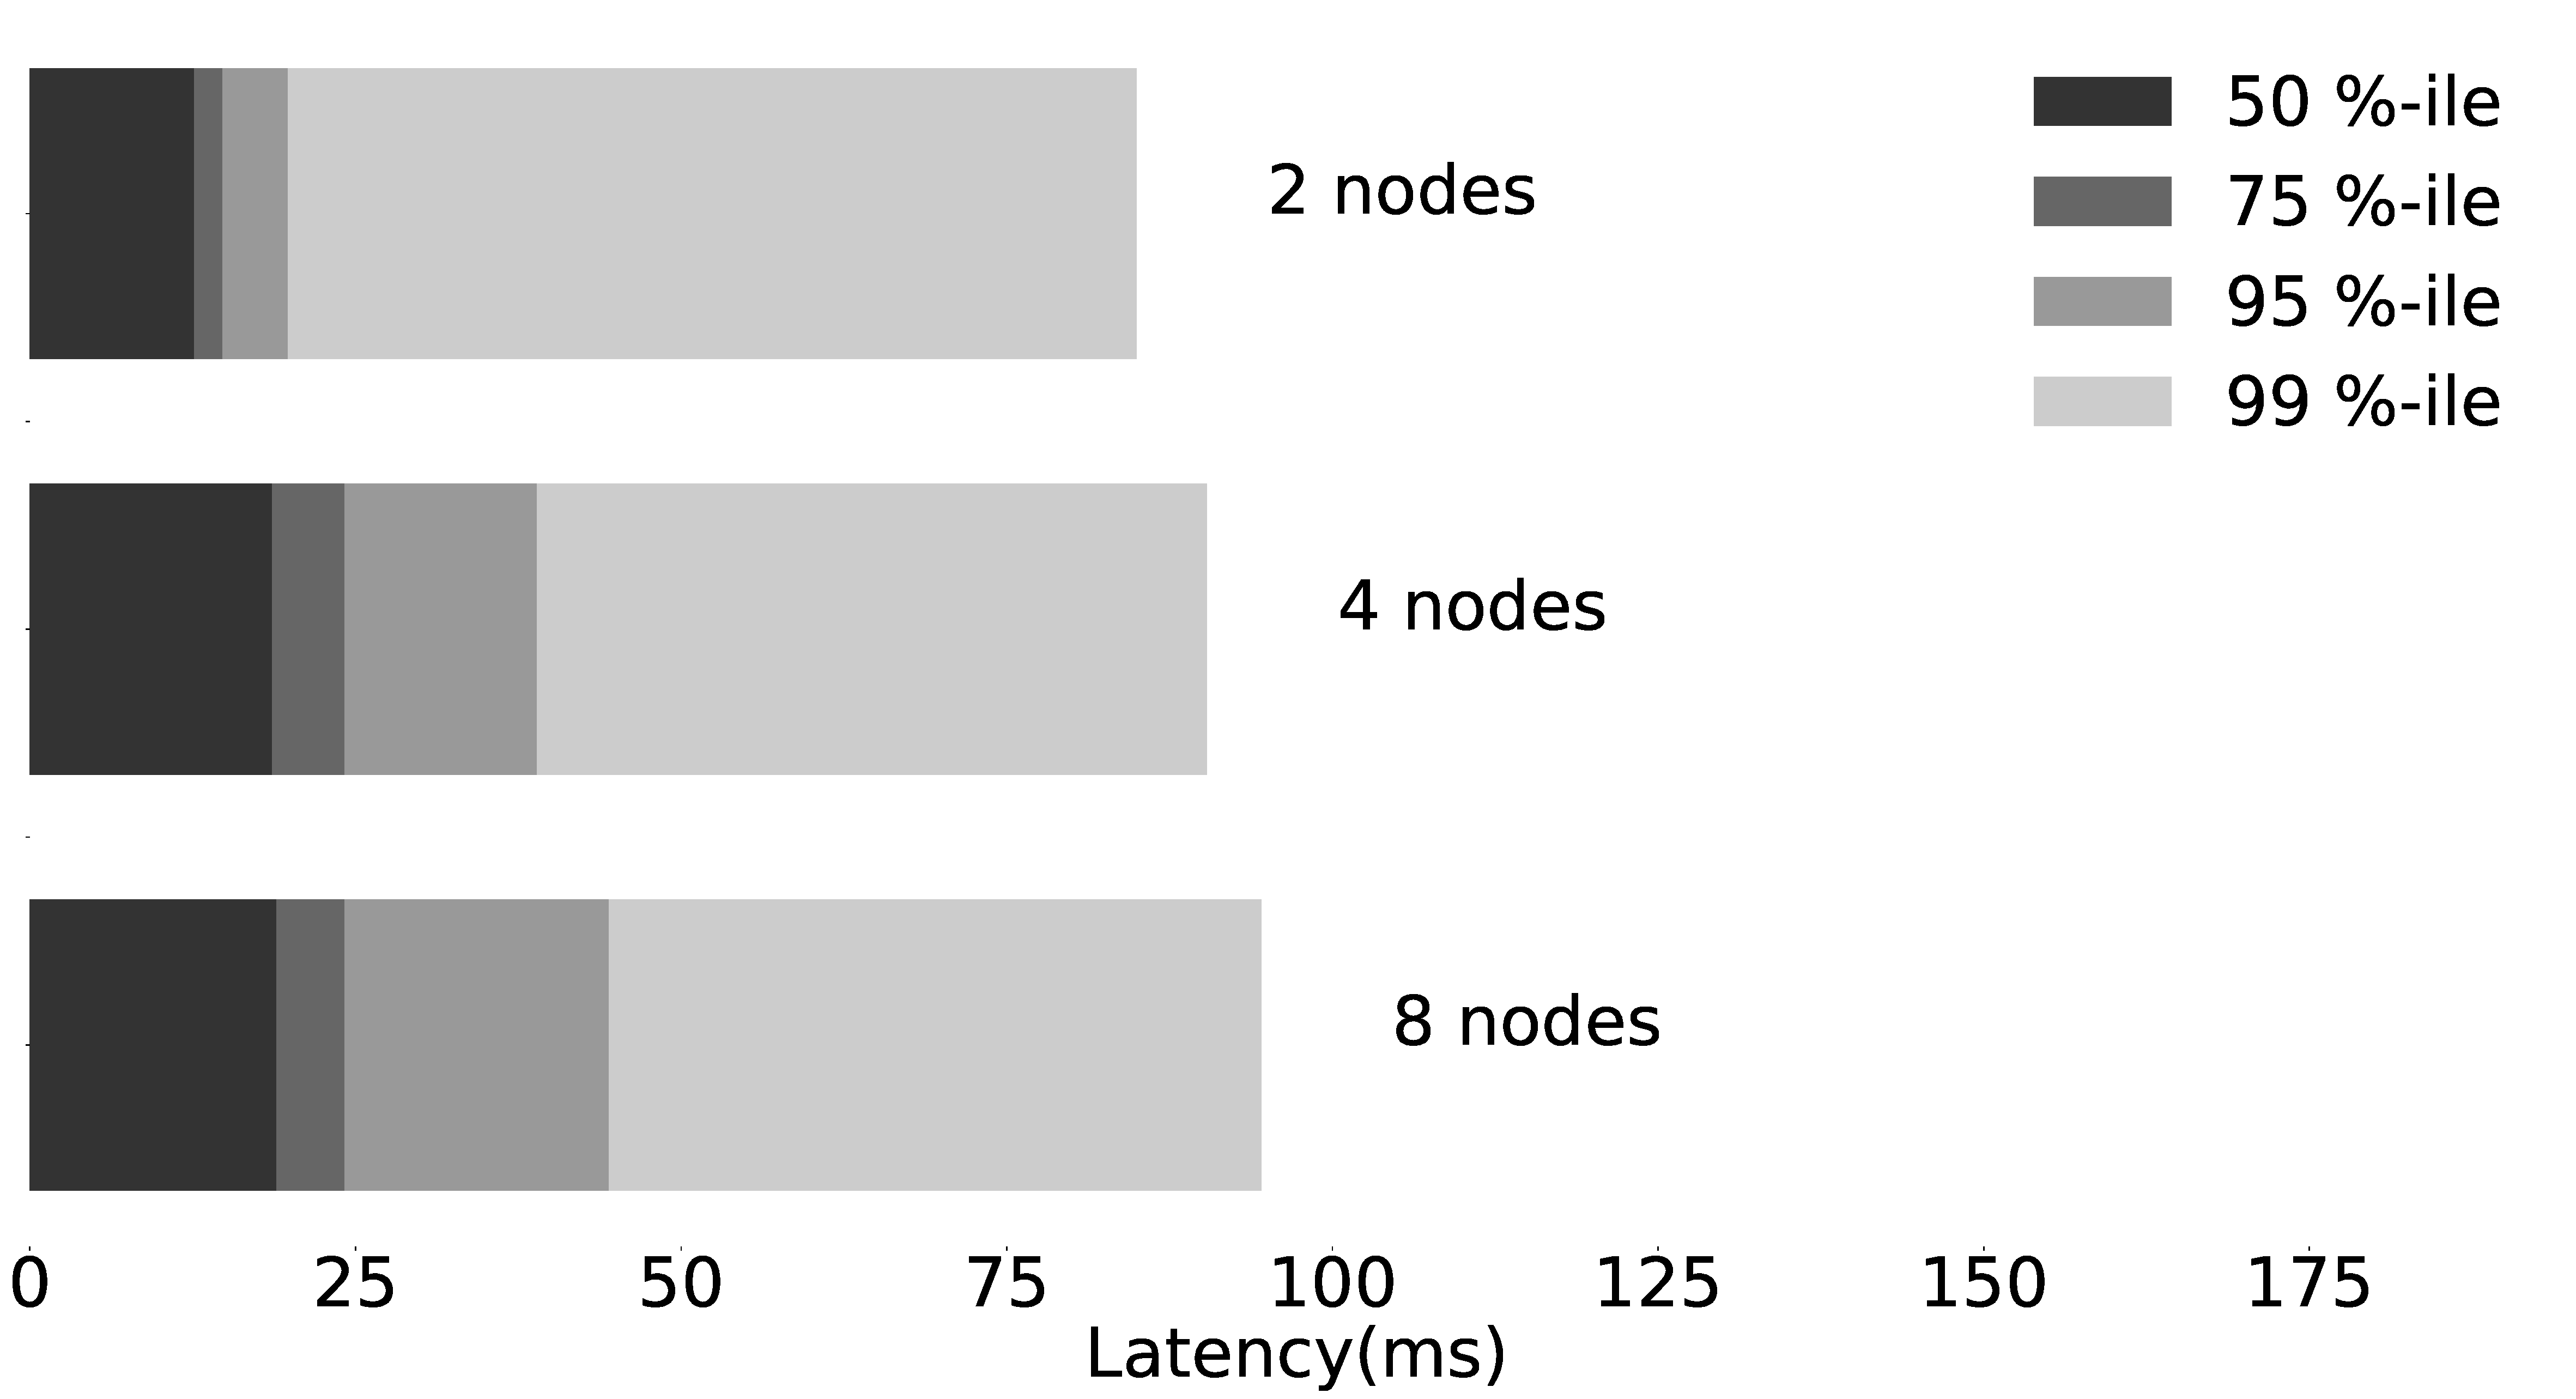
\includegraphics[scale=0.1]{pics/classifier_latencies}
  \caption{Classifier latencies}
  \label {latencies}
\end{figure}

We launched FlameStream on different clusters, containing 2, 4 and 8 nodes respectively. The clusters tested workload of 10000 lenta.ru documents. It is expected a linear increase in performance, however, in reality, it is hardly achievable. Figure ~\ref{latencies} shows, that mean latency of classifier prediction is less than 25 ms. Figure ~\ref{throughput} illustrates the system's linear throughput increase, where 8 machines are able to handle 100 docs per second.

\begin{figure}[htbp]
  \centering
  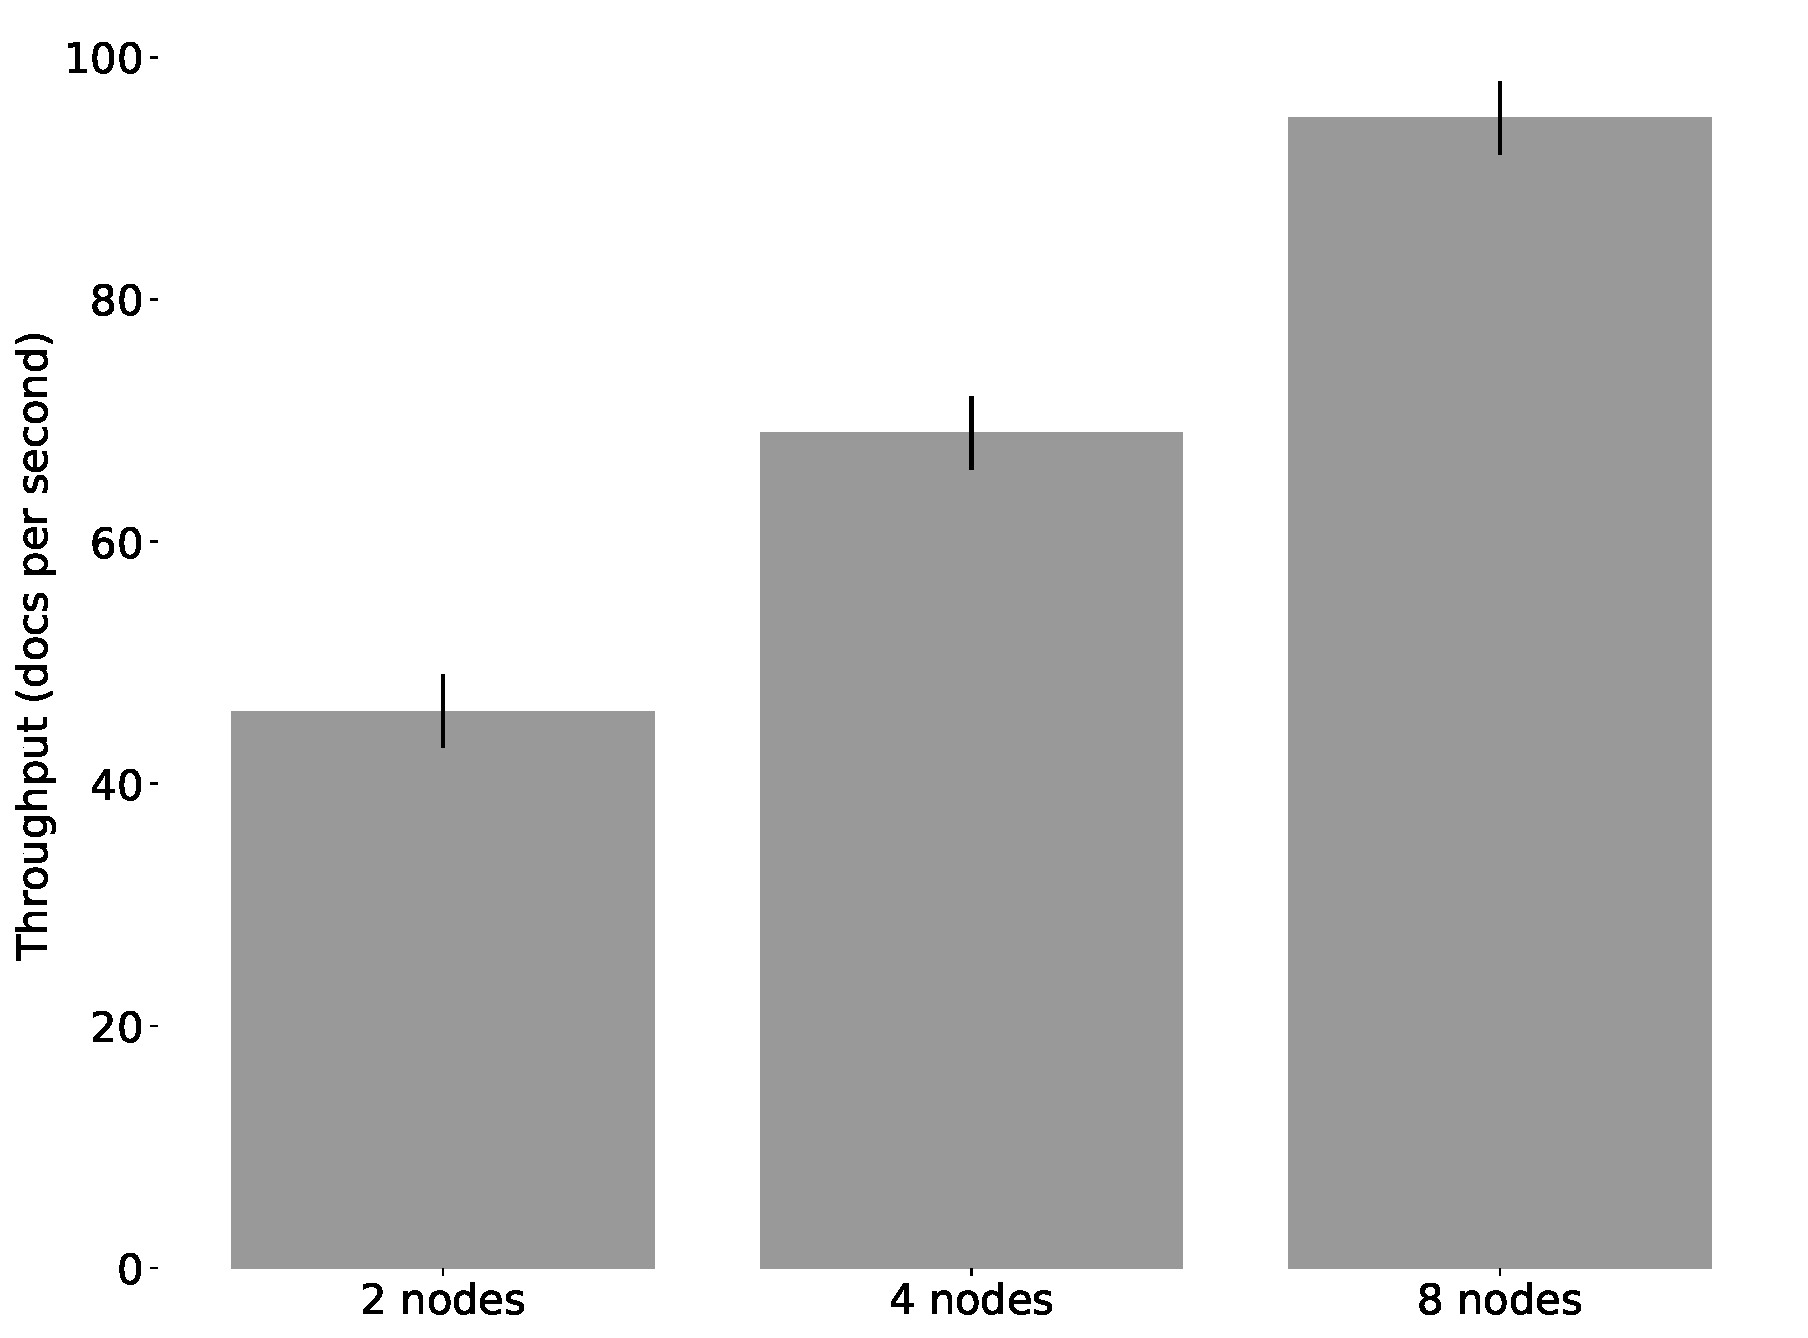
\includegraphics[scale=0.2]{pics/classifier_throughput}
  \caption{Classifier throughput}
  \label {throughput}
\end{figure}